\section{Захват людей на изображении и оценка их позы}

\subsection{Введение}
\subsection{Математическая модель}

Чтобы достичь надёжного захвата людей благоразумно взять модель тела, которая предпологает, что оно (тело) состоит из частей. Обозначим их конфигурацию как \(L = \{l_o, l_1, \dots, l_N\}\), где состояние части \(i\) определено как \(l_i = (x_i, y_i, \theta_i, s_i)\). \(x_i\) и \(y_i\) -- позиция цетра части в координатах изображения, \(\theta_i\) -- её расположение, \(s_i\) -- масштаб, который подсчитывается относительно размера частей из тренировочного набора данных.

В зависимости от задачи число частей объекта может изменяться. Например, для захвата верхней части тела можно использовать модель из 6 частей: голова, торс, левая и правая кисти, левое и правое предплечья. В случае захвата всего человека следует добавать в предыдущую модель еще 4 части: левое и правое бедра, левую и правую голени.

Имея наблюдение \(D\) апостериорная вероятность конфигурации частей \(L\) моделируется как \(\rho(L{\mid}D)\propto\rho(D{\mid}L)\rho(L)\), где \(\rho(D{\mid}L)\) -- вероятность наблюдения при конкретной конфигурации частей. В методе, использующем графический структуры (pictorial structures), \(\rho(L)\) соответствует априорное кинематическое дерево (\emph{kinematic tree prior}). Обе состовляющие могут быть получены через обучение на тренировочном наборе данных.

Использую вышеприведенную модель, можно оценить позы, если найти наиболее вероятные положения каждой из частей нахождением максимума \(\rho(l_i{\mid}D)\). В случае нескольких людей на изображении, следует искать моды распределения.

\begin{figure}
  \centering
  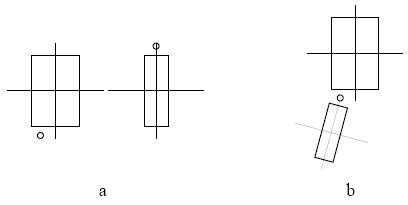
\includegraphics[width=0.6\textwidth]{images/detection-two-parts.png}
  \caption{Две части сочлененного объекта, (a) в своих координатах и (b) наилучшая конфигурация частей\label{detection-two-parts}}
\end{figure}

\subsubsection{Априорное кинематическое дерево}

Первым существенным компонентом в методе графических структур является \(\rho(L)\), которая кодирует вероятностные ограничения на конфигурацию частей. Источником таких ограничений является кинематические связи между частями. После отображения кинематической структуры на направленный ацикличный граф (directed acyclic graph, DAG), распределение вероятностей конфигураций может быть представлено как:
\begin{equation}
  \rho(L) = \rho(l_0)\prod_{(i,j){\in}E}\rho(l_i{\mid}l_j),
\end{equation}
где \(E\) -- множество всех направленных ребер в кинематическом дереве, \(l_0\) -- корень дерево (в нашем случае, торс человека).

\emph{Связи частей}. Для того, чтобы завершить определение априорного распределения, следует определить все составляющие уравнения (1). Распределение для конфигурации корневой части \(\rho(l_0)\) предполагается равномерным, что позволяет применять эту модель ко множеству разнообразных конфигураций. Связи частей моделируются с помощью нормальных распределений, который способствуют эффективному выводу. Это может показаться существенным ограничением данной модели, так как, например, распределение расположения кисти при данном положении предплечья представляет собой полукруг (это интуитивно понятно), а не форму нормального распределения.

Однако, как было показано в \cite{felzenszwalb05}, хоть данное распределение и не является нормальным в координатах изображения, возможно преобразовать его в другое пространство, в котором пространственное распределение между частями будет прекрасно описыватться нормальным распределением. Говоря формально, для моделирования \(\rho(l_i{\mid}l_j)\) следует преобразовать конфигурацию части \(l_i = (x_i, y_i, \theta_i, s_i)\) в координатную систему соединений между двумя частями, используя следующее преобразование:
\begin{equation}
  T_{ji}(l_i) =
  \begin{pmatrix}
    x_i + s_id_x^{ji}\cos{\theta_i} - s_id_y^{ji}\sin{\theta_i}\\
    y_i + s_id_x^{ji}\sin{\theta_i} - s_id_y^{ji}\cos{\theta_i}\\
    \theta_i + \tilde{\theta}_{ji}\\
    s_i
  \end{pmatrix}.
\end{equation}

Здесь \(d^{ji} = (d_x^{ji}, d_y^{ji})^T\) -- средняя относительная позиция соединения частей \(i\) и \(j\) в координатной системе части \(i\), \(\tilde{\theta}_{ji}\) -- относительный угол между частями. Тогда отношение частей моделируется нормальным распределением в полученном пространстве:
\begin{equation}
  \rho(l_i{\mid}l_j) = N(T_{ji}(l_i){\mid}T_{ij}(l_j), \Sigma^{ji}),
\end{equation}
где \(T_{ij}\) -- преобразование, которое отображает позицию предшествующей части \(l_j\) в расположение соединения между частями \(i\) и \(j\), \(\Sigma^{ji}\) -- ковариация между частями, которая была извлечена из тренировочного набора данных, который определяет жёсткость соединения. Также нужно извлечь среднюю относительную позицию соединения \(d^{ji}\). \(d^{ji}\) и \(\Sigma^{ji}\) могут быть извлечены методом максимального правдоподобия (maximum likelihood estimation).

\subsubsection{Извлеченные модели частей}

\begin{figure}
  \centering
  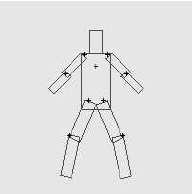
\includegraphics[width=0.4\textwidth]{images/detection-learned-body.png}
  \caption{Конфигурация тела человека, извлеченная из тренировочных примеров\label{detection-learned-body}}
\end{figure}

Другим важным компонентом является вероятность \(\rho(D{\mid}L)\) наблюдения \(D\), имея конфигурацию \(L\). Мы полагаемся на специфичные для каждой части модели внешнего вида, каждая из которых представлена в виде \(d_i\), которая сообщает о наблюдении части \(i\) в каждой возможной позиции, масштабе и повороте. Чтобы унифицировать диффиринцирующую модель внешнего вида с порождающей моделью объекта, мы предпологаем, что наблюдения (\emph{evidences}) частей формируются, основываясь на знании истинной конфигурации объекта \(L\). Предположим, что наблюдения частей (\emph{part evidences}) условно независимы при данной конфигурации \(L\) и что \(d_i\) для части \(i\) зависит только от своей собственной конфигурации \(l_i\), тогда выражение вероятности предстанет в следующем виде:
\begin{equation}
  \rho(D{\mid}L) = \prod_{i = 0}^N\rho(d_i{\mid}L) = \prod_{i = 0}^N\rho(d_i{\mid}l_i).
\end{equation}

Хоть это и слишком упрощающее допущение, оно оправданно до тех пор, пока части не заслоняют друг друга значительно. Более того, такая формулировка позволяет делать точный и эффективный вывод. Как следствие из уравнения (4), апостериорная вероятность конфигураций частей может быть представлена как:
\begin{equation}
  \rho(L{\mid}D) \propto \rho(l_0) \prod_{i = 0}^N\rho(d_i{\mid}l_i) \prod_{(i, j) \in E}\rho(l_i{\mid}l_j).
\end{equation}

\emph{Встреченные проблемы}. В ходе разработки модели были рассмотрены некоторые соображения, которые повлияли на её итоговый вид. Цель данной разработки -- захватывать и оценивать позу объектов в средах без искусственных ограничений. Так как пространство поиска всех возможных поз, как правило, очень велико, то редукция пространства поиска может оказать огромную помощь. Как известно, использование дифференцирующих детекторов позволяет значительно редуцировать пространство поиска для порождающей модели, тем самым предоставляя не только быстрый, но и точный вывод в сложных сценах из реального мира.

Также важно избегать преждевременную фильтрацию возможнных позиций частей на стадии детектирования частей и откладывать окончательное решение до тех пор, пока наблюдение всех частей не станет доступно. Поэтому мы производим обширный поиск и рассматриваем все возможные позиции, расположения и масштабы.

\emph{Усиленные детекторы частей}

\subsubsection{Точный вывод модели}

Важным свойством такой деревоподобной модели является то, что вывод вычислим в разумное время. Например, мы можем подсчитать глобально оптимальную конфигурацию с помощью метода максимального правдопободия (maximum a posteriori estimation, MAP), используя алгортм максимального произведения (\emph{max-product algorithm}). Более того, мы можем подсчитать точное маржинальное распределение (marginal distribution) с помощью sum-product алгоритма.

Также можно интерпретировать направленную графическую модель как factor graph и применить стандартный factor graph belief propagation (sum-product алгоритм).

Важным наблюдением является тот факт, что если зависимости частей моделируются нормальным распределением, тогда дорогостоящее суммирование в sum-product алгоритме может быть эффективно подсчитано с помощью свертки Гаусса. Но следует делать это осторожно, так как связи частей в нашей модели Гауссовы не с пространстве изображения, а в преобразованном пространстве соединений частей.

И все же чтобы применить алгортм эффективно, мы преобразуем сообщения в координатную систему соединений частей с помощью уравнения (2), а затем применяем свертку Гаусса, и наконец, преобразуем результат в координатную систему целевой части.

\begin{figure}
  \centering
  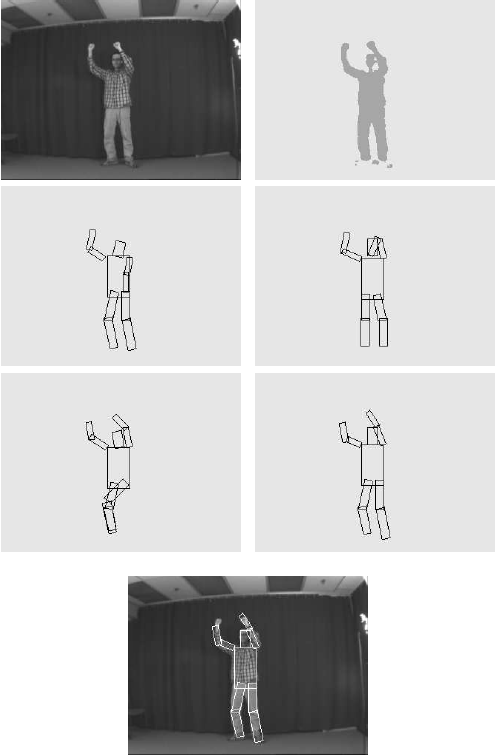
\includegraphics[width=0.8\textwidth]{images/detection-stages.png}
  \caption{Исходное изображение, бинарное изображение, случайные выборки апостериорного распределения конфигурации, лучшая выборка\label{detection-stages}}
\end{figure}

\begin{figure}
  \centering
  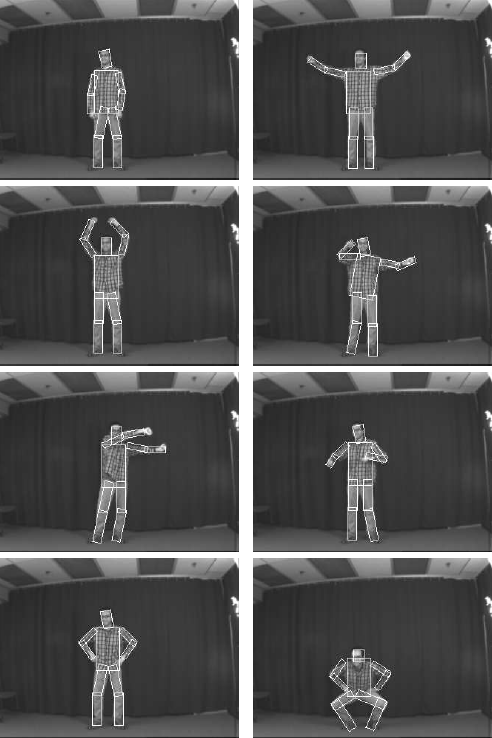
\includegraphics[width=0.8\textwidth]{images/detection-matching-results.png}
  \caption{Результаты захвата\label{detection-matching-results}}
\end{figure}

\begin{figure}
  \centering
  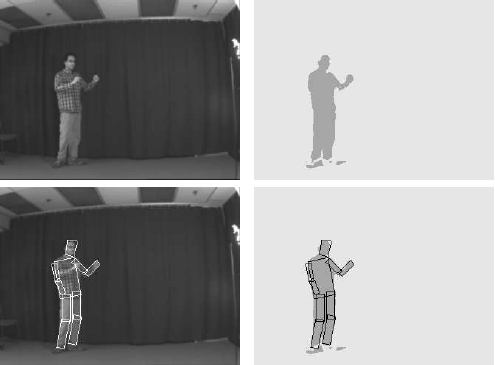
\includegraphics[width=0.8\textwidth]{images/detection-not-enough-info.png}
  \caption{Бинарное изображение не содержит достаточно информации для оценки позиции кисти\label{detection-not-enough-info}}
\end{figure}

\begin{figure}
  \centering
  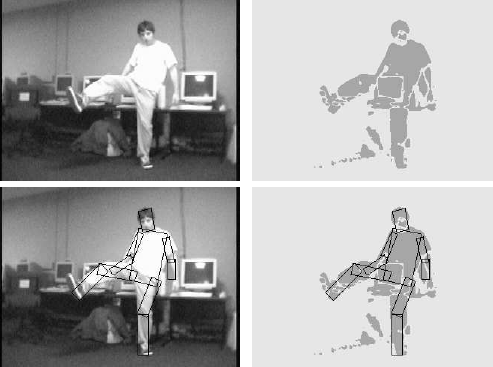
\includegraphics[width=0.8\textwidth]{images/detection-noisy.png}
  \caption{Демонстрация работы с зашумленными данными\label{detection-noisy}}
\end{figure}

\begin{figure}
  \centering
  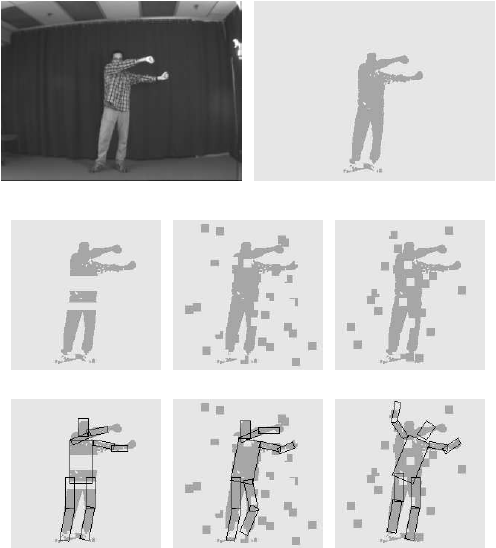
\includegraphics[width=0.8\textwidth]{images/detection-corrupted.png}
  \caption{Результаты захвата на поврежденном изображении\label{detection-corrupted}}
\end{figure}

\newpage
